\documentclass[11pt]{article}

\usepackage{amsmath}
\usepackage{amsfonts}
\usepackage{amsthm}
\usepackage{blkarray}
\usepackage{caption}
\usepackage{enumitem}
\usepackage{hyperref}
\usepackage{mathtools}
\usepackage{tikz}
\usepackage[top=1.5cm,bottom=2cm,left=1.25cm,right=1.75cm,marginparwidth=1.75cm]{geometry}
\setlength{\parindent}{0cm}

\newcommand{\N}{\mathbb{N}}
\newcommand{\R}{\mathbb{R}}
\newcommand{\C}{\mathbb{C}}
\newcommand{\n}{\vspace{0.3cm}}
\newtheorem{theorem}{Theorem}

\def\lc{\left\lceil}
\def\rc{\right\rceil}
\def\lf{\left\lfloor}
\def\rf{\right\rfloor}

\title{\vspace{-1.0cm}CSCI 5304 Homework 4}
\author{Fletcher Gornick}
\date{November 9, 2023}

\begin{document}
\maketitle
\begin{enumerate}
	\item \begin{enumerate}
		      \item Show that a real \(n \times n\) matrix \(A\) (not necessarily symmetric) is positive definite iff \(\frac12(A + A^T)\) is SPD.
		            \begin{proof}
			            Let \(x\) be any nonzero vector,
			            \begin{align*}
				            \left(\frac12(A + A^T)x, x \right) > 0
				             & \iff \frac12 x^T(A + A^T)x > 0              & \text{(constants can be pulled out)} \\
				             & \iff \frac12 x^T Ax + \frac12 x^T A^T x > 0 & (\text{distribution of vectors})     \\
				             & \iff \frac12(Ax, x) + \frac12(x, Ax) > 0    & (\text{definition of inner product}) \\
				             & \iff \frac12(Ax, x) + \frac12(Ax, x) > 0    & (\text{symmetry of inner product})   \\
				             & \iff (Ax, x) > 0.
			            \end{align*}
			            Since \(\left(\frac12 (A + A^T),x \right) > 0 \text{ iff } (Ax,x) > 0\) for all nonzero \(x\), we can conclude the above statement holds.
		            \end{proof}

		      \item Find a \(2 \times 2\) real matrix which satisfies \((Ax,x) > 0\) for all \textit{real} nonzero vectors \(x\), but which is not positive definite when regarded as a member of \(\C^{2 \times 2}\).
		            \[(Ax,x) = x^TAx = (x_1 \; x_2) \begin{pmatrix} a_{11} & a_{12} \\ a_{21} & a_{22} \end{pmatrix} \binom{x_1}{x_2} = a_{11}x_1^2 + a_{12}xy + a_{21}xy + a_{22}y^2,\]
		            So if we choose \(A = \begin{pmatrix} 1 & 1 \\ -1 & 1 \end{pmatrix}\), we see that \((Ax,x) = x_1^2 + x_2^2 > 0\) for all \(x \in \R^2\), but if we treat \(A\) as complex, we can take \(x = \binom1i\), and we get
		            \[(Ax,x) = a_{11} \bar x_1 x_1 + a_{21} x_1 \bar x_2 + a_{12} \bar x_1 x_2 + a_{22} \bar x_2 x_2 = 1 \cdot 1 \cdot 1 -1 \cdot 1 \cdot (-i) + 1 \cdot 1 \cdot i + 1 \cdot (-i) \cdot i = 2 + 2i \not \in \R\]
		            Since there's an \(x \in \C\), \(x \neq 0\) such that \((Ax,x) \not \in \R\), we know \(A\) cannot be positive definite in the complex sense.
	      \end{enumerate} \n

	\item Let \(A \in \R^{n \times n}\) be a symmetric positive definite matrix.
	      \begin{enumerate}
		      \item Show that \(|a_{ij}| < \sqrt{a_{ii}a_{jj}}\)
		            \begin{proof}
			            Since \(A\) SPD, we know there exists \(m \times n\) matrix \(G\) such that \(A = G^T G\), so we can calculate \(a_{ij}\) like so:
			            \[a_{ij}^2 = \left( \sum_{k=1}^m (G^T)_{ik}(G)_{kj} \right)^2 = \left( \sum_{k=1}^m g_{ki}g_{kj} \right)^2 \leq \left( \sum_{k=1}^m g_{ki}^2 \right) \left( \sum_{k=1}^m g_{kj}^2 \right) = a_{ii}a_{jj} \]

			            The inequality from above was an application of the Cauchy-Schwarz inequality.  This isn't exacly what we want though, we still must show that \(|a_{ij}| \neq \sqrt{a_{ii}a_{jj}}\), so let's take vector \(x \in \R^n\) consisting of all zeros, except \(x_i = \sqrt{a_{jj}}, \; x_j = -\sqrt{a_{ii}}\), and assume \(a_{ij} = \sqrt{a_{ii}a_{jj}}\).  This yields:
			            \[(Ax,x) = x^T A x = \textstyle\sum\limits_{k=1}^n \textstyle\sum\limits_{\ell=1}^n x_k a_{k \ell} x_\ell = x_{ii}^2a_{ii} + x_{jj}^2a_{jj} - 2x_ix_ja_{ij} = a_{jj}a_{ii} + a_{ii}a_{jj} - 2\sqrt{a_{ii}}\sqrt{a_{jj}}\sqrt{a_{ii}a_{jj}} = 0.\]
			            Therefore it also cannot be the case that \(|a_{ij}| = \sqrt{a_{ii}a_{jj}}\), and we can conclude \(|a_{ij}| < \sqrt{a_{ii}a_{jj}}\) if \(A\) is symmetric positive definite.
		            \end{proof}

		      \item Show that \(|a_{ij}| < (a_{ii}+a_{jj})/2\)
		            \begin{proof}
			            If we take \(x = e_i - e_j\), we get the following value for \((Ax,x)\):
			            \[(Ax,x) = x_i^2a_{ii} + x_j^2a_{jj} - 2x_ix_ja_{ij} = a_{ii} + a_{jj} - 2a_{ij}.\]
			            Since \(A\) is SPD, \(a_{ii} + a_{jj} - 2a_{ij} > 0 \implies a_{ij} < (a_{ii}+a_{jj})/2\).  Similarly, taking \(x = e_i + e_j\) yields \(-a_{ij} < (a_{ii}+a_{jj})/2\).  Therefore, we can conclude \(|a_{ij}| < (a_{ii}+a_{jj})/2\).
		            \end{proof}
	      \end{enumerate}

	\item Show that the following symmetric matrices are not positive definite.
	      \[
		      A = \begin{pmatrix} 0 & 3 & 1 \\ 3 & 2 & 0 \\ 1 & 0 & 2 \end{pmatrix}, \quad
		      B = \begin{pmatrix} 2 & 3 & 1 \\ 3 & 2 & 0 \\ 1 & 0 & 2 \end{pmatrix}, \quad
		      C = \begin{pmatrix} 1 & 0 & 2 \\ 0 & 2 & 0 \\ 2 & 0 & 2 \end{pmatrix}.
	      \]
	      \begin{proof}
		      For matrix \(A\), we see \(a_{11} = 0\), so if we simply take \(e_1\), we see \(e_1^T A e_1 = 0\). \n\\
		      For matrix \(B\), we see \(b_{11} = b_{22} = 2\) and \(b_{12} = 3\), but \(b_{12} = 3 \geq 2 = \sqrt{b_{11}b_{22}}\), this violates the statement proven in 2(a), so we can conclude \(B\) cannot be positive definite. \n\\
		      Similarly, in matrix \(C\), we see \(c_{11} = 1,  c_{33} = 2,\) and \(c_{13} = 2\).  These values also violate the statement proven in 2(a), so we can again confirm \(C\) is not SPD (via contrapositive).
	      \end{proof}

	\item The Hald cement data is used in several books and papers as an example of regression and least-squares.  The right-hand side is the heat evolved in cement during hardening.  The variables are coefficients \(\xi_1, \dots, \xi_4\) of four different ingredients of the mix.  The right-hand side \(b\) and the matrix \(A \in \R^{13 \times 4}\) can be found in the matlab section on the class web-site.  To \(\xi_1, \dots, \xi_4\) we add a constant (\(\xi_0\)) to the model.  In effect, we want to find \(\xi_0, \xi_1, \dots, \xi_4\) so that \(\xi_0 + \xi_1 a_{i,1} + \cdots + \xi_4 a_{i,4} \approx b_i\) for \(i=1:13\).
	      \begin{enumerate}
		      \item Solve the least squares problem to get the \(\xi_i\)'s by the method of normal equations.  What is \(\kappa_2(A)\)?
		            \[
			            Fx \approx b \to (1 : A)x \approx b \to
			            \begin{pmatrix}
				            1 & 7  & 26 & 6  & 60 \\
				            1 & 1  & 29 & 15 & 52 \\
				            1 & 11 & 56 & 8  & 20 \\
				            1 & 11 & 31 & 8  & 47 \\
				            1 & 7  & 52 & 6  & 33 \\
				            1 & 11 & 55 & 9  & 22 \\
				            1 & 3  & 71 & 17 & 6  \\
				            1 & 1  & 31 & 22 & 44 \\
				            1 & 2  & 54 & 18 & 22 \\
				            1 & 21 & 47 & 4  & 26 \\
				            1 & 1  & 40 & 23 & 34 \\
				            1 & 11 & 66 & 9  & 12 \\
				            1 & 10 & 68 & 8  & 12
			            \end{pmatrix}
			            \begin{pmatrix}
				            \xi_0 \\ \xi_1 \\ \xi_2 \\ \xi_3 \\ \xi_4
			            \end{pmatrix}
			            \approx
			            \begin{pmatrix}
				            78.5 \\ 74.3 \\ 104.3 \\ 87.6 \\ 95.9 \\ 109.2 \\ 102.7 \\ 72.5 \\ 93.1 \\ 115.9 \\ 83.8 \\ 113.3 \\ 109.4
			            \end{pmatrix}
		            \]
		            Using normal equations to minimize the difference between \(Fx\) and \(b\), we get
		            \[F^T Fx \;=\; F^T b \implies x \;=\; (F^T F)^{-1} F^T b \;=\; (62.4054, 1.5511, 0.5102, 0.1019, -0.1441)^T\]
		            For calculating the condition number, \(\kappa_2(A) = \lVert A \rVert_2 \lVert A^+ \rVert_2\) where \(A^+ = (A^T A)^{-1} A^T\) is the pseudo-inverse of \(A\).  Plugging into julia, we get
		            \[\kappa_2(A) \;=\; \verb$opnorm(A,2) * opnorm(pinv(A),2)$ \;=\; 20.5846.\]

		      \item We now show how to get rid of the constant unknown from the system.  Write \(x = \binom{\xi_0}{y}\) where \(\xi_0\) is a scalar, and show how to eliminate \(\xi_0\) from the system.  The resulting problem is now a least-squares problem of the form \(\min \lVert By-c \rVert_2\) involving only the \(y\) vector.  Show the matrix \(B\) and new right-hand side \(c\).  What is the condition number of \(B\)? \n\\
		            To eliminate \(\xi_0\) from the system, it's as simple as removing the constant vector of \(\xi_0\)'s:
		            \[Fx =
			            \begin{pmatrix}
				            \xi_0 + a_{1,1}\xi_1 + \cdots + a_{1,4}\xi_4 \\
				            \xi_0 + a_{2,1}\xi_1 + \cdots + a_{2,4}\xi_4 \\
				            \vdots                                       \\
				            \xi_0 + a_{13,1}\xi_1 + \cdots + a_{13,4}\xi_4
			            \end{pmatrix}
			            =
			            \begin{pmatrix} \xi_0 \\ \xi_0 \\ \vdots \\ \xi_0 \end{pmatrix} +
			            \begin{pmatrix}
				            a_{1,1}\xi_1 + \cdots + a_{1,4}\xi_4 \\
				            a_{2,1}\xi_1 + \cdots + a_{2,4}\xi_4 \\
				            \vdots                               \\
				            a_{13,1}\xi_1 + \cdots + a_{13,4}\xi_4
			            \end{pmatrix}
			            = \bar{\xi_0} + Ay.
		            \]
		            So if we let \(B = A = F(:,2:5)\), then we get \(By \approx b - \bar\xi_0\), so \(c = b - \bar\xi_0\), and since \(B = A\) in this case, \(\kappa_2(B) = \kappa_2(A) = 20.5846\). \n

		      \item Continued from (b).  How can you interpret \(c\) relative to \(b\) and \(B\) relative to \(A\)? \n\\
		            From (b), we see \(B = A\), and \(c = b - \bar\xi_0\) (meaning each \(c_i = b_i - \xi_0\)), so
		            \[\lVert By - c \rVert_2 = \lVert Ax_{(1:4)} - b + \xi_0 \rVert_2.\]
	      \end{enumerate} \n

	\item The purpose of this exercise is to test 3 ways of computing the QR factorization of the matrix \(A\);
	      \begin{enumerate}
		      \item The classical Gram-Schmidt algorithm
		      \item The modified Gram-Schmidt algorithm
		      \item The Cholesky factorization of \(A^T A\)
	      \end{enumerate}

	      Explain how the Cholesy factorization of \(A^T A\) can be used.  In the following, you should us the script \verb!cholR! that's posted.  You can use \verb!inv! to invert triangular matrices. \n\\
	      The Cholesky factorization gives us a fast method of finding \(R\).  Suppose we use \verb$cholR(A'A)$ and find that \(G^T G = A^T A\), we now see
	      \[G^T G = A^T A = (QR)^T QR = R^T Q^T QR = R^T R \implies G = R,\]
	      \begin{minipage}{0.65\textwidth}
		      so it must be the case that \(G\) is one potential \(R\) in the QR decomposition because they're both upper-triangular.  Now, since we know \(G = R\), we have \(A = QG \implies Q = AG^{-1}\). \n

		      The script to the right calculates QR decomposition utilizing the Cholesky factorization.
	      \end{minipage}
	      \begin{minipage}{0.35\textwidth}
		      \begin{verbatim}
     function cholQR(A)
       R = cholR(A'*A)
       Q = A * inv(R)
       Q, R
     end
        \end{verbatim}
	      \end{minipage} \n

	      A data set is posted on the class web-site.  Write a script which loads the matrix and then for each of the three methods above, compute the \(Q\) and \(R\) factors and the error measures
	      \[\lVert A - Q * R \rVert_2, \quad \lVert I - Q^T * Q \rVert_2.\]
	      Present your results in the form of a table and comment on them.
	      \begin{verbatim}
results = Matrix{Float64}(undef,2,3)     |    results[1,1] = norm(M - Q1*R1)
M = readdlm(file, ' ', Float64, '\n')    |    results[1,2] = norm(M - Q2*R2)
                                         |    results[1,3] = norm(M - Q3*R3)
Q1, R1 = cgsa(M)                         |    results[2,1] = norm(I[1:5,1:5] - Q1'*Q1)
Q2, R2 = mgsa(M)                         |    results[2,2] = norm(I[1:5,1:5] - Q2'*Q2)
Q3, R3 = cholQR(M)                       |    results[2,3] = norm(I[1:5,1:5] - Q3'*Q3)\end{verbatim}
	      \def\arraystretch{1.5}
	      \begin{center}\begin{tabular}{|c||c|c|c|}
			      \hline
			      RESULTS                       & Classical Gram-Schmidt     & Modified Gram-Schmidt      & Cholesky Factorization     \\
			      \hline\hline
			      \(\lVert A - QR \rVert_2\)    & \(2.1499 \times 10^{-16}\) & \(1.3878 \times 10^{-16}\) & \(3.4276 \times 10^{-16}\) \\
			      \hline
			      \(\lVert I - Q^T Q \rVert_2\) & 0.0093                     & \(6.5811 \times 10^{-10}\) & 0.0949                     \\
			      \hline
		      \end{tabular}\end{center}
	      All three methods result in a decomposition with \(QR\) sufficiently close to \(A\) (all within a factor of \(10^{-16}\) off).  Notably, the Cholesky factorization method is still about twice as bad as the other two.

	      The modified Gram-Schmidt method performs significantly better when computing orthogonal matrix \(Q\).  Classical Gram-Schmidt has calculated error around 0.01, and the Choleskey factorization method has an error of about 0.1, so it seems that the modified Gram-Schmidt wins this round.

	\item We saw in class that if \(w \in \R^n\) and \(\lVert w \rVert_2 = 1\), then the matrix \(P = I - 2ww^T\), called a Householder reflector, is at the same time symmetric and unitary.  Let \(x \in \R^n\), with \(x \neq 0\), and let \(y = Px\).
	      \begin{enumerate}
		      \item When do we have \(y = x\)? \n\\
		            When \(x\) is within the hyperplane span\(\{w\}^\perp\).  If \(x\) is already in this plane, then applying householder reflector \(P\) to \(x\) won't change anything.  So \(y = Px = x \iff (x,w) = 0\). \n

		      \item Assume now that \(w^T x > 0\).  Show that \(y \neq x\) and that \(w = (x-y)/\lVert x-y \rVert_2\). \n\\
		            First, it's clear to see that \(w^T x > 0 \iff y \neq x\):
		            \[x - y = x - Px = x - (I - ww^T)x = x - x + ww^T x = \alpha w \;\; (\alpha = w^T x > 0).\]
		            Since \(x - y \neq 0\), we know \(y \neq x\).  Now, to show \(w = (x-y)/\lVert x-y \rVert_2\), remember that \(w\) is a unit vectore, and \(\alpha > 0\) from above:
		            \[\frac{x-y}{\lVert x-y \rVert_2} = \frac{\alpha w}{\lVert \alpha w \rVert_2} = \frac{\alpha w}{|\alpha| \lVert w \rVert_2} \frac{w}{\lVert w \rVert_2} = w.\]

		      \item Show a geometric illustration of the result in (b). \\
		            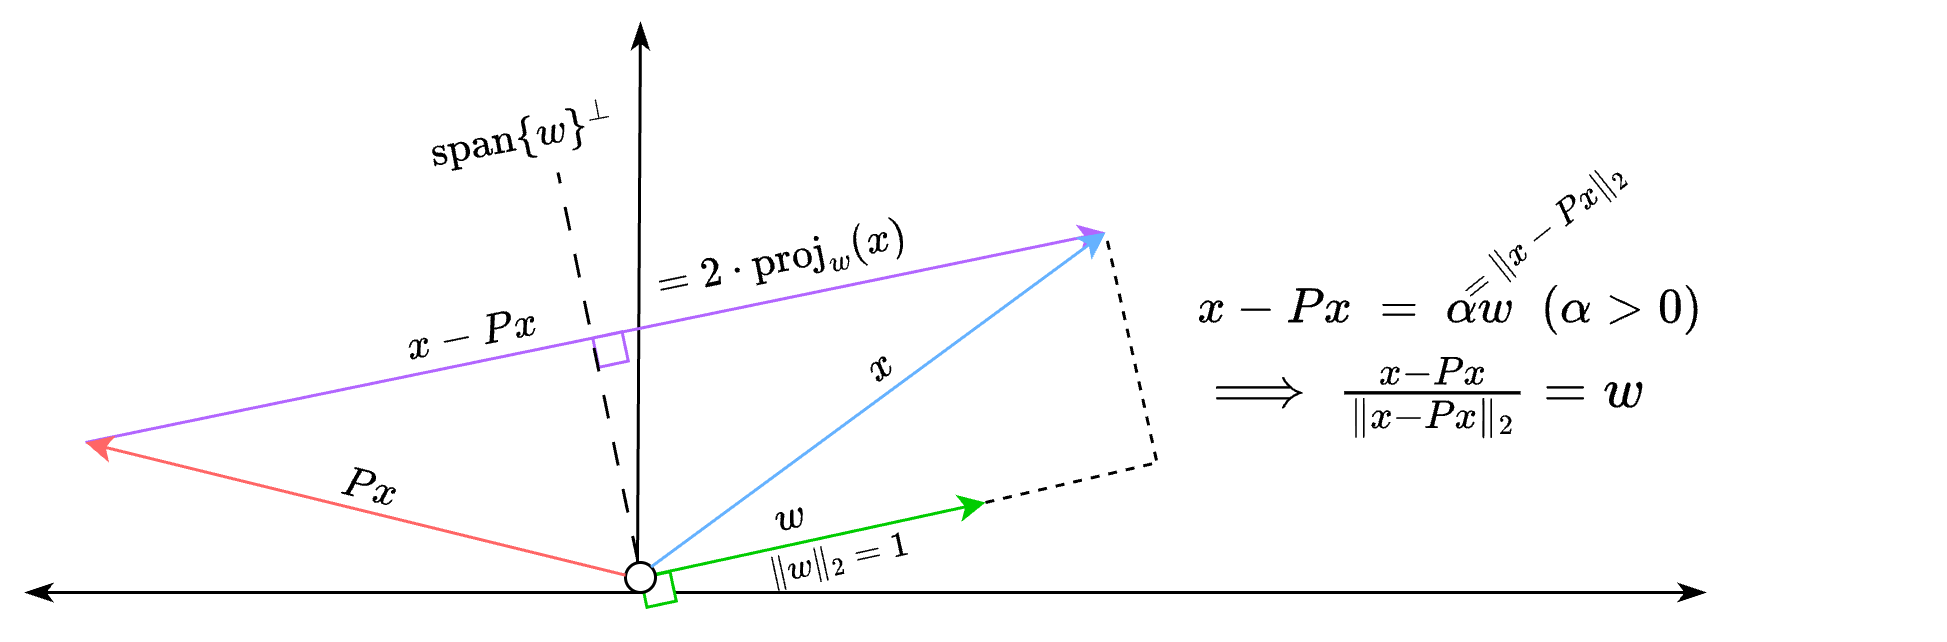
\includegraphics[width=\textwidth]{householder.png}
	      \end{enumerate}

	\item Implement a julia function which computes the Householder QR factorization of a full rank matrix \(A\).  The function should look like:
	      \[\verb!V, bet = houseQR(A)!\]
	      where \verb!V! is the matrix of vectors \(v_1, \dots, v_m\) that are related to the successive Householder reflectors \(P_j = I - \beta_j v_j v_j^T\) used to transform \(A\) into upper triangular form, and \verb!bet! is the vector of coefficients \(\beta_j\).  Show the julia function. \n\\
	      Script on next page.
	      \footnotesize
	      \begin{verbatim}
                                                  |   function house1(x)
using LinearAlgebra                               |     m = size(x)[1]
using DelimitedFiles                              |     m == 1 && return 1, 0
                                                  |
function house(X)                                 |     v = [1 ; x[2:m]]
  X = deepcopy(X)                                 |     sigma = v[2:m]' * v[2:m]
  m,n = size(X); V = zeros(m,n); bet = zeros(n)   |
                                                  |     if (sigma == 0)
  for k = 1 : n                                   |       bet = 0
    S = X[k:m,k:n]                                |     else
    v,b = house1(S[:,1])                          |       xnrm = sqrt(x[1]^2 + sigma)
                                                  |       v[1] = (x[1] <= 0 ? x[1] - xnrm : x[1] + xnrm)
    X[k:m,k:n] = S - b * v * v' * S               |
    V[k:m,k] = v; bet[k] = b                      |       bet = 2 / (1+sigma/v[1]^2)
  end                                             |       v = v / v[1]
                                                  |     end
  V, bet                                          |
end                                               |     v, bet
                                                  |   end
        \end{verbatim}
	      \normalsize

	\item Test the program developed above for the same data as the one used for Question 5 above.  Obtain the \(Q_1, R_1\) matrices of the factorization \(A = Q_1R_1\) - where \(Q_1\) is \(m \times n\) and \(R_1\) is \(n \times n\), from the Householder factorization.  Compare the \(R_1\) matrix obtained from the Householder method with the \(R\) matrix obtained from the Modified Gram-Schmidt method seen in Question 5 (\(\lVert R_1 - R \rVert_1\)).  Similarly, compute the norms \(\lVert I - Q^T Q \rVert_1\) and \(\lVert I - Q_1^T Q_1 \rVert_1\).
    \begin{verbatim}
                          function house_qr(X)
                            V, bet = house(X)
                            m = size(V)[1]; n = size(bet)[1]
                            eye = Float64.(I[1:m,1:m])
                            Q = eye; R =  deepcopy(X)
                          
                            for j = 1 : n
                              k = n + 1 - j
                          
                              Rp = R[j:m,j:n]; v = V[j:m,j]; b = bet[j]
                              R[j:m,j:n] = Rp - b * v * v' * Rp
                              R[j+1:m,j] = zeros(m-j)
                          
                              v = V[:,k]; b = bet[k]
                              Q = Q - b * v * v' * Q
                            end
                            Q, R
                          end
\end{verbatim}
    I used the above script to retrieve the QR factorization from our householder function, then got the thin decomposition by taking \(Q_1 = Q[:,1:n], \; R_1 = R[1:n,:]\).  From this, I got the following norms:
    \[\lVert R_1 - R \rVert_2 = 2.7519 \times 10^{-14}, \quad \lVert I - Q^T Q \rVert_2 = 7.2599 \times 10^{-16} \quad \lVert I - Q_1^T Q_1 \rVert_2 = 3.2045 \times 10^{-16}.\]
\end{enumerate}
\end{document}
